\documentclass[11pt]{article}

\oddsidemargin=0in
\evensidemargin=0in
\textwidth=6.3in
\topmargin=-0.5in
\textheight=9in

\parindent=0in
%\pagestyle{empty}


\def\changemargin#1#2{\list{}{\rightmargin#2\leftmargin#1}\item[]}
\let\endchangemargin=\endlist 

%------------------------------------------------------------------
% PROBLEM, PART, AND POINT COUNTING...

% Create the problem number counter.  Initialize to zero.
\newcounter{problemnum}

% Specify that problems should be labeled with arabic numerals.
\renewcommand{\theproblemnum}{\arabic{problemnum}}


% Create the part-within-a-problem counter, "within" the problem counter.
% This counter resets to zero automatically every time the PROBLEMNUM counter
% is incremented.
\newcounter{partnum}[problemnum]

% Specify that parts should be labeled with lowercase letters.
\renewcommand{\thepartnum}{\arabic{partnum}}

% Make a counter to keep track of total points assigned to problems...
\newcounter{totalpoints}

% Make counters to keep track of points for parts...
\newcounter{curprobpts}		% Points assigned for the problem as a whole.
\newcounter{totalparts}		% Total points assigned to the various parts.

% Make a counter to keep track of the number of points on each page...
\newcounter{pagepoints}
% This counter is reset each time a page is printed.

% This "program" keeps track of how many points appear on each page, so that
% the total can be printed on the page itself.  Points are added to the total
% for a page when the PART (not the problem) they are assigned to is specified.
% When a problem without parts appears, the PAGEPOINTS are incremented directly
% from the problem as a whole (CURPROBPTS).


%---------------------------------------------------------------------------


% The \problem environment first checks the information about the previous
% problem.  If no parts appeared (or if they were all assigned zero points,
% then it increments TOTALPOINTS directly from CURPROBPTS, the points assigned
% to the last problem as a whole.  If the last problem did contain parts, it
% checks to make sure that their point values total up to the correct sum.
% It then puts the problem number on the page, along with the points assigned
% to it.

\newenvironment{problem}[1]{
% STATEMENTS TO BE EXECUTED WHEN A NEW PROBLEM IS BEGUN:
%
% Increment the problem number counter, and set the current \ref value to that
% number.
\refstepcounter{problemnum}
%
% Add some vspace to separate from the last problem.
\vspace{0.15in} \par
%
\setcounter{curprobpts}{#1} \setcounter{totalparts}{0}	% Reset counters.
%
% Now put in the "announcement" on the page.
\noindent{\Large \bf Question \theproblemnum. \normalsize ({\it \arabic{curprobpts} point\null\ifnum \value{curprobpts} = 1\else s\fi}\/)}
}{
% STATEMENTS TO BE EXECUTED WHEN AN OLD PROBLEM IS ENDED:
%
% If no parts to problem, then increment TOTALPOINTS and PAGEPOINTS for the
% entire problem at once.
\ifnum \value{totalparts} = 0
	\addtocounter{totalpoints}{\value{curprobpts}}	% Add pts to total.
	\addtocounter{pagepoints}{\value{curprobpts}}	% Add pts to page total.
%
% If there were parts for the problem, then check to make sure they total up
% to the same number of points that the problem is worth. Issue a warning
% if not.
\else \ifnum \value{totalparts} = \value{curprobpts}
	\else \typeout{}
	\typeout{!!!!!!!   POINT ACCOUNTING ERROR   !!!!!!!!}
	\typeout{PROBLEM [\theproblemnum] WAS ALLOCATED \arabic{curprobpts} POINTS,}
	\typeout{BUT CONTAINS PARTS TOTALLING \arabic{totalparts} POINTS!}
	\typeout{}
	\fi
\fi
}


%---------------------------------------------------------------------------


% The \newpart command increments the part counter and displays an appropriate
% lowercase letter to mark the part.  It adds points to the point counter
% immediately.  If 0 points are specified, no point announcement is made.
% Otherwise, the announcement is in scriptsize italics.

\newcommand{\newpart}[2]{
\refstepcounter{partnum}	% Set the current \ref value to the part number.
\begin{changemargin}{0in}{0in}
  \noindent\textbf{\theproblemnum.\thepartnum}~(\textit{#1 points}): 
  \textit{ #2}
\end{changemargin}
\addtocounter{totalparts}{#1}	% Add points to totalparts for this problem.
\addtocounter{pagepoints}{#1}	% Add points to total for this page.
\addtocounter{totalpoints}{#1}	% Add points to total for entire test.
}

\newcommand{\answerpart}[1]{
\begin{changemargin}{0.25in}{0in}
\noindent \textbf{Answer:} {#1}
\end{changemargin}	
}

\newcommand{\answer}[1]{
\textbf{Answer:} {#1}
}



%---------------------------------------------------------------------------



% Just in case you want to skip some numbers in your test...

\newcommand{\skipproblem}[1]{\addtocounter{problemnum}{#1}}



%---------------------------------------------------------------------------


% The \showpoints command simply gives a count of the total points read in up to
% the location at which the command is placed.  Typically, one places one
% \showpoints command at the end of the latex file, just prior to the
% \end{document} command.  It can appear elsewhere, however.

\newcommand{\showpoints}
{
\typeout{}
\typeout{====> A TOTAL OF \arabic{totalpoints} POINTS WERE READ.}
\typeout{}
}


%---------------------------------------------------------------------------



\usepackage{graphicx}
\usepackage[english]{babel}
\usepackage[latin1]{inputenc}
\usepackage{times}
\usepackage[T1]{fontenc}
\usepackage{amsmath}
\usepackage{amssymb}
\usepackage{subfigure}

\newcommand{\argmax}{\mathop{\arg\max}}
\newcommand{\deriv}[1]{\frac{\partial}{\partial {#1}} }
\newcommand{\dsep}{\mbox{dsep}}
\newcommand{\Pa}{\mathop{Pa}}
\newcommand{\ND}{\mbox{ND}}
\newcommand{\De}{\mbox{De}}
\newcommand{\Ch}{\mbox{Ch}}
\newcommand{\graphG}{{\mathcal{G}}}
\newcommand{\graphH}{{\mathcal{H}}}
\newcommand{\setA}{\mathcal{A}}
\newcommand{\setB}{\mathcal{B}}
\newcommand{\setS}{\mathcal{S}}
\newcommand{\setV}{\mathcal{V}}
\DeclareMathOperator*{\union}{\bigcup}
\DeclareMathOperator*{\intersection}{\bigcap}
\DeclareMathOperator*{\Val}{Val}
\newcommand{\mbf}[1]{{\mathbf{#1}}}
\newcommand{\eq}{\!=\!}

\newcommand{\discrete}{stripes}
\newcommand{\gaussian}{swirl}

\newcommand{\attention}[1]{\marginpar{\sl\raggedright \bf #1}}

\usepackage{ascii}
\usepackage[T1]{fontenc}

\begin{document}

{\centering
  \rule{6.3in}{2pt}
  \vspace{1em}
  {\Large
    CS688: Graphical Models - Spring 2020\\
    Assignment 4\\
  }
  \vspace{1em}
  Assigned: Wed, Apr 8th. Due: Mon, Apr 20th, 11:59am. \\
  \vspace{0.1em}
  \rule{6.3in}{1.5pt}
}\vspace{1em}

\textbf{General Instructions:} Submit a report with the answers to each question at the start of class on the date the assignment is due. You are encouraged to \emph{typeset your solutions}. For your assignment to be considered ``on time'', you must upload a zip file containing all of your code to Gradescope by the due date. Make sure the code is sufficiently well documented that it's easy to tell what it's doing. You may use any programming language you like. For this assignment, you may \textbf{not} use existing code libraries for inference with CRFs or MRFs, or any code library for sampling. If you think you've found a bug with the data or an error in any of the assignment materials, please post a question to the Piazza discussion forum. Make sure to list in your report any outside references you consulted (books, articles, web pages, etc.) and any students you collaborated with.\\

\textbf{Academic Honesty Statement:} Copying solutions from external sources (books, web pages, etc.) or other students is considered cheating. Sharing your solutions with other students is also considered cheating. Any detected cheating will result in a grade of -100\% on the assignment for all students involved, and potentially a grade of F in the course.\\

\textbf{Introduction:} In this part, you will experiment with Monte Carlo Inference. 
More specifically, you will experiment with Monte Carlo image denoising using grid-structured conditional random field models.\\

\textbf{Binary Model:} Consider a probability distribution over a vector $y \in \{-1,+1\}^d$ model of the form

\[ p(y \vert b,w) = \frac{1}{Z} \prod_{i=1}^d \exp( b_i y_i ) \prod_{(i,j)\in \text{pairs}} \exp(w_{ij} y_i y_j). \]

Here, each component $y_i$ of $y$ is in $\{-1,+1\}$, we can think of the ``bias" $b_i$ as ``how much $y_i$ wants to be $+1$", and we can think of the weights $w_{ij}$ as ``how much $y_i$ and $y_j$ want to have the same value".

\begin{problem}{5} \textbf{Derivation of conditional distribution}
Mathematically derive a formula for $p(y_i = 1 \vert y_{-i}, b, w)$, the conditional probability that $y_i=1$ given the state of all other variables. Write your solution using the function $\sigma(s) := 1/(1+\exp(-s))$. You will need to reference the set of all neighbors of $i$, $\text{nb}(i)$. 
\end{problem}
\\

\begin{problem}{5} \textbf{Pseudo-Code for Gibbs Sampling}
Write pseudo-code for the Gibbs sampling algorithm, where in each iteration, you update for $i=1,i=2,...,i=d$. (This is slightly different from in class where each iteration used a single randomly chosen $i$.) You should take as input (1) the total number of iterations, and (2) the model parameters $\{b, w\}$. You should return a list of the samples of $y$ that you get after each iteration.
\end{problem}
\\

\begin{problem}{5} \textbf{Samples}
Consider an $30 \times 30$ 4-connected grid structured model where we have a zero bias of $b_i=0$, and a constant interaction strength of $w_{ij}=\bar{w}$.  Now, implement the Gibbs sampling algorithm. For each value of $\bar{w} \in \{0, .1, .2, .3, .4, .5\}$, run a single chain Markov chain for 100 iterations. (Where, again, one iteration is a full pass over the entire grid.) Plot the final samples for each $\bar{w}$ value. Show each sample as an image with black pixels for variables with $y_i=-1$ and white pixels for variables with for $y_i=+1$. Make sure to label each image with the value of $\bar{w}$ it corresponds to.
\end{problem}
\\

\begin{problem}{5} \textbf{Discussion}
Explain briefly (no more than a single paragraph of 4 sentances) why the images from the previous question look like they do, and why they change for various values of $\bar{w}$.
\end{problem}
\\


\begin{problem}{5} \textbf{ Mixing Times}
For the model in the previous problem, it is easy to see by symmetry that the true mean value of $y$ is $\mathbb{E}[y]=0$. To get an idea of average performance, for each value of $\bar{w} \in \{0, .1, .2, .3, .4, .5\}$ run \emph{100 independent} Markov chains each for 100 iterations. (Where, again, one iteration is a full pass over the entire grid). For each iteration, compute the mean value of $y$ (averaged over the 100 independent repetitions).
Plot the 6 curves together on one graph, with the number of iterations on the x-axis and the mean value of $y$ on the y-axis. Make sure to label the axes and the value of $\bar{w}$ for each curve.
\end{problem}
\\

\begin{problem}{5} \textbf{Discussion}
Do your samples give the correct value of $\mathbb{E}[y]$? When do the samples look better or worse? Explain in a single paragraph of no more than four sentences why the curves in the previous problem look as they do.
\end{problem}
\\

\textbf{Data Set:} The data for the remaining questions consists of a single $200 \times 154$ pixel binary image.  The original image is {\asciifamily im\_clean.png}, while the copy with noise is {\asciifamily im\_noisy.png}.
The two images are shown below. We will refer to the images on the left as the ``true" image and the image with noise as the ``observed" or ``noisy" image.

\begin{figure}[ht]
\centering
\subfigure[im\_clean]{
   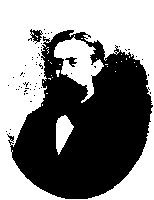
\includegraphics[width=1.1in] {Figures/im_clean.png}
 }
 \subfigure[im\_noisy]{
   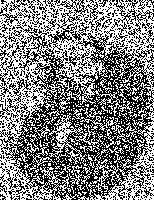
\includegraphics[width=1.1in] {Figures/im_noisy.png}
 }
\label{fig:faces}
\end{figure}



\textbf{Image Denoising Model: } Intuitively, given a ``noisy image" $x$, we should think of this defining a probabilistic model over the ``clean image'' $y$, with the structure shown in the figure on the next page.

\begin{figure}[ht]
\centering
   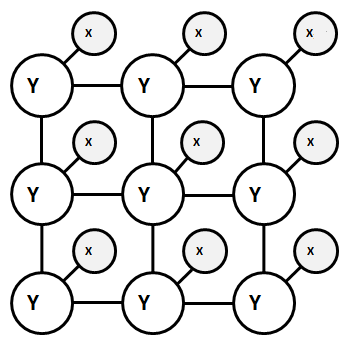
\includegraphics[width=3in] {Figures/grid-crf.png}
\label{fig:crf}
\end{figure}

We can think of the model as being defined exactly as in the previous problem, except that $b(x,\theta)$ and $w(x,\theta)$ are now functions of the input $x$ as well as some parameters $\theta$

\[ p(y \vert x, \theta) = \frac{1}{Z(x)} \prod_{i=1}^d \exp( b_i(x,\theta ) y_i ) \prod_{(i,j)\in \text{pairs}} \exp(w_{ij}(x,\theta ) y_i y_j). \]


\begin{problem}{10} \textbf{Fixed Parameter Denoising}
Make sure you scale the input $x$ so that each value is either -1 or +1. Then, determine the parameters by the simple mapping of $b_i = .5 x_i$ and $w_{ij}=0.3$. Run 100 iterations of Gibbs sampling. Show an image of $\mu$, the mean value of $y$ you obtain over those samples, and report the mean per-pixel absolute difference of $\mu$ from the true output. (Make sure to scale your image appropriately so that all values between $-1$ and $+1$ are shown, and make sure that both $\mu$ and $y$ are in the original space between $-1$ and $+1$ before computing a difference.)
\end{problem}

\begin{problem}{10} \textbf{Varying Parameters}
Consider setting $b_i = \theta_1 x_i$ and $w_{ij} = \theta_2$ where $\theta_1$ and $\theta_2$ are 2 unknown parameters. (In the previous problem we essentially used $\theta_1 = .5$ and $\theta_2 = 0.3$) Can you find a pair of $\theta_1$ and $\theta_2$ to give you lower error than the values from the previous problem? Limit the total number of iterations you do for any parameter setting to 100 iterations. Describe (a) how you tried to find better parameters (there is no single correct answer here) (b) show an image of your final denoised image and (c) report the final error.
\end{problem}
\\


{\bf Extra Credit} Finally, here are some extra-credit problems. These are \emph{far} more difficult than the above problems and have very small point values. \emph{These problems are a terrible "value" in terms of the points you will earn for spending your time}. To maximize your score with limited time, you should make sure the above problems are done thoroughly and ignore these.  We will be very stingy in giving credit for these problems- do them only for the glory, and at your own risk! These problems are more open-ended. As a result, you will need to carefully describe what you did for each problem.

\begin{problem}{5} \textbf{MCMC: Varying $w_{ij}$ parameters}
Come up with a scheme to have $w_{ij}$ vary as a function of $x$, rather than being constant. (1) Describe the informal motivation for the scheme (2) describe formally what you have done (3) Give an image of the final results (4) list your final error, and how much this improves on the previous problem.
\end{problem}
  
\begin{problem}{5} \textbf{MCMC: Faster mixing}
Above, we used a fixed update order of $s=1,2,...,d$. Can you come up with a different update order that leads to faster mixing? (Meaning that you get closer to the true mean value of $0$ during the 100 iterations. (1) Describe what your improved update order is and (2) make another version of the same graph from Question 5, showing your improvement. (3) Discuss why you think this mixes faster.
\end{problem}
  
%\showpoints
\end{document} 
